\documentclass[11pt,a4paper]{article}
\usepackage[utf8]{inputenc}\usepackage[T1]{fontenc}\usepackage{mathptmx}\usepackage[scaled=0.9]{helvet}\usepackage{courier}
\usepackage[margin=2.3cm]{geometry}\usepackage{amsmath,amssymb}\usepackage{graphicx}
\usepackage{booktabs}\usepackage{listings}\usepackage{xcolor}\usepackage{fancyhdr}
\usepackage[hidelinks]{hyperref}\usepackage{caption}\usepackage{tikz}
\usetikzlibrary{positioning,arrows.meta}
\renewcommand{\contentsname}{Table des matières}
\renewcommand{\figurename}{Figure}\renewcommand{\tablename}{Tableau}
\pagestyle{fancy}\fancyhf{}
\lhead{\small Blombou -- Bouaboud -- Nanda -- Sissoko -- Ziani}\rhead{\small SIT213 -- Rapport Étape 3}\cfoot{\thepage}
\lstset{basicstyle=\ttfamily\small,columns=fullflexible,breaklines=true,frame=single,backgroundcolor=\color{gray!6},literate={é}{{\'e}}1{è}{{\`e}}1{à}{{\`a}}1{É}{{\'E}}1}
\newcommand{\EbNo}{E_b/N_0}
\sloppy\setlength{\parskip}{4pt}\setlength{\parindent}{0pt}
\begin{document}
\begin{titlepage}\centering
{\large IMT Atlantique -- FIP2A\\ Module SIT213\par}\vspace{3cm}
{\LARGE\bfseries Simulation d'une chaîne de transmission numérique\par}\vspace{0.6cm}
{\Large Rapport -- Étape 3\\[4pt]\normalsize Transmission non idéale sur canal à bruit blanc additif gaussien\par}\vspace{2.5cm}
\begin{tabular}{rl}
Groupe : & B4 -- FIP2A\\[4pt]
Auteurs : & BLOMBOU Ethan\\ & BOUABOUD Anis-Melwan\\ & NANDA Laurent\\ & SISSOKO Mohamed Djoncounda\\ & ZIANI Mohamed Amine\\[4pt]
Date : & Septembre 2026
\end{tabular}\vfill
\end{titlepage}
\tableofcontents\newpage

\section{Objectifs de l'étape 3}
L'étape 3 remplace le canal analogique parfait de l'étape 2 par un canal à \textbf{bruit blanc additif gaussien} (BBAG, ou AWGN). Le signal émis n'arrive plus intact au récepteur : des erreurs de décision apparaissent et le taux d'erreur binaire (TEB) devient non nul. L'objectif est donc de :
\begin{itemize}
  \item modéliser le canal $r(n) = s(n) + b(n)$ avec $b(n)\sim\mathcal N(0,\sigma_b^2)$ ;
  \item régler $\sigma_b^2$ à partir du rapport signal à bruit par bit $\EbNo$ fourni en paramètre ;
  \item vérifier que le bruit généré est bien gaussien ;
  \item tracer le TEB en fonction de $\EbNo$ et le confronter aux prévisions théoriques.
\end{itemize}

\section{Chaîne implémentée}
\begin{figure}[h]\centering
\resizebox{\linewidth}{!}{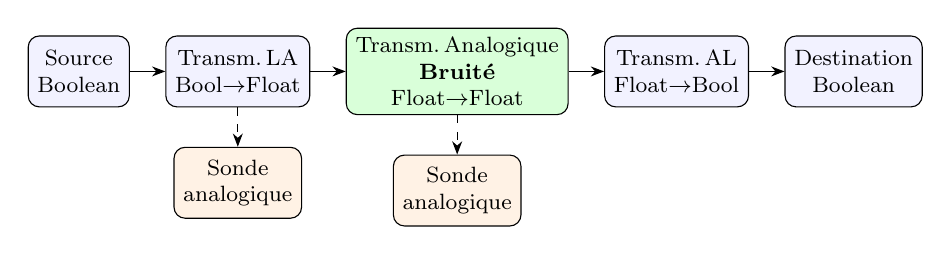
\begin{tikzpicture}[node distance=0.45cm,b/.style={draw,rounded corners,align=center,font=\footnotesize,minimum height=0.9cm,fill=blue!5},>=Stealth]
\node[b] (s) {Source\\Boolean};
\node[b,right=of s] (e) {Transm.\,LA\\Bool$\to$Float};
\node[b,right=of e,fill=green!15] (c) {Transm.\,Analogique\\\textbf{Bruité}\\Float$\to$Float};
\node[b,right=of c] (r) {Transm.\,AL\\Float$\to$Bool};
\node[b,right=of r] (d) {Destination\\Boolean};
\draw[->] (s)--(e); \draw[->] (e)--(c); \draw[->] (c)--(r); \draw[->] (r)--(d);
\node[b,below=0.5cm of e,fill=orange!10] (s1) {Sonde\\analogique}; \draw[->,dashed] (e)--(s1);
\node[b,below=0.5cm of c,fill=orange!10] (s2) {Sonde\\analogique}; \draw[->,dashed] (c)--(s2);
\end{tikzpicture}}
\caption{Chaîne de l'étape 3 -- seul le canal (en vert) change par rapport à l'étape 2.}
\end{figure}
L'architecture en composants connectables mise en place aux étapes 1 et 2 a permis d'introduire le bruit sans modifier ni l'émetteur (\texttt{TransmetteurLogiqueAnalogique}) ni le récepteur (\texttt{TransmetteurAnalogiqueLogique}) : le simulateur instancie simplement un \texttt{TransmetteurAnalogiqueBruite} à la place du \texttt{TransmetteurAnalogiqueParfait} lorsque l'option \texttt{-snrpb} est présente.

\section{Prévisions avant simulation}
\subsection{Paramètres pertinents}
\begin{center}\begin{tabular}{lll}\toprule
Paramètre & Option & Rôle\\\midrule
Rapport $\EbNo$ (dB) & \texttt{-snrpb} & fixe la puissance du bruit\\
Forme d'onde & \texttt{-form} & NRZ, NRZT ou RZ\\
Nombre d'échantillons par bit $N$ & \texttt{-nbEch} & intervient dans le calcul de $\sigma_b^2$\\
Amplitudes $A_{\min}, A_{\max}$ & \texttt{-ampl} & fixent la puissance $P_s$ et le seuil\\
Longueur du message & \texttt{-mess} & précision statistique du TEB\\
Semence & \texttt{-seed} & reproductibilité (message et bruit)\\\bottomrule
\end{tabular}\end{center}

\subsection{Résultats attendus}
\begin{itemize}
  \item Le TEB doit décroître de façon monotone quand $\EbNo$ augmente, et tendre vers $0{,}5$ quand $\EbNo\to-\infty$.
  \item Le TEB doit être indépendant de l'amplitude absolue du signal : multiplier $A_{\min}$ et $A_{\max}$ par un même facteur multiplie $P_s$, donc $\sigma_b$, dans le même rapport.
  \item Pour un récepteur optimal (filtre adapté), la théorie donne $\text{TEB} = Q\big(\sqrt{2\EbNo}\big)$ en NRZ antipodal et $Q\big(\sqrt{\EbNo}\big)$ pour un signal unipolaire (0, $A$), soit une pénalité de 3~dB pour l'unipolaire.
  \item Notre récepteur de l'étape 2 ne prend qu'\textbf{un seul échantillon par bit}. On s'attend donc à des performances inférieures à la borne optimale ; la section~\ref{sec:analyse} quantifie cet écart.
\end{itemize}

\section{Modélisation du canal gaussien}
\subsection{Réglage de la puissance du bruit}
D'après la séance 3, en notant $P_s$ la puissance moyenne du signal, $T$ la durée d'un bit, $F_e$ la fréquence d'échantillonnage et $N = TF_e$ le nombre d'échantillons par bit :
\[
E_b = P_s T,\qquad N_0 = \frac{2\sigma_b^2}{F_e}
\quad\Longrightarrow\quad
\frac{E_b}{N_0} = \frac{P_s\,N}{2\sigma_b^2}.
\]
On inverse cette relation pour obtenir la variance du bruit à appliquer :
\[
\boxed{\sigma_b^2 = \frac{P_s\,N}{2\cdot 10^{(\EbNo)_{\text{dB}}/10}}}
\]
La puissance $P_s$ est estimée directement sur le signal reçu par le canal, $P_s = \frac1K\sum_{n=1}^{K}s^2(n)$, ce qui la rend automatiquement correcte quelle que soit la forme d'onde et les amplitudes choisies.

\subsection{Génération du bruit}
Chaque échantillon de bruit est obtenu à partir de deux tirages uniformes indépendants $a_1, a_2\sim\mathcal U[0,1[$ (transformation de Box--Muller donnée en cours) :
\[ b(n) = \sigma_b\sqrt{-2\ln\big(1-a_1(n)\big)}\,\cos\big(2\pi a_2(n)\big). \]
L'utilisation de $1-a_1$ plutôt que $a_1$ évite le calcul de $\ln 0$, puisque \texttt{nextDouble()} peut renvoyer exactement 0.

\subsection{Classe \texttt{TransmetteurAnalogiqueBruite}}
\begin{itemize}
  \item Hérite de \texttt{Transmetteur<Float, Float>}.
  \item Constructeur \texttt{(int nbEch, float ebN0Db, Integer seed)} : le générateur \texttt{java.util.Random} est initialisé avec la semence si l'option \texttt{-seed} est fournie, ce qui permet de rejouer une simulation à l'identique.
  \item \texttt{emettre()} : calcule $P_s$, en déduit $\sigma_b$, ajoute un échantillon de bruit à chaque échantillon du signal puis transmet le résultat aux destinations connectées. Un message vide est retransmis tel quel.
\end{itemize}

\subsection{Nouvelle option du simulateur}
\begin{center}\begin{tabular}{ll}\toprule Option & Description\\\midrule
\texttt{-snrpb s} & canal bruité, $\EbNo = s$ dB (flottant, peut être négatif) ; active le mode analogique\\\bottomrule\end{tabular}\end{center}
Sans cette option, le canal reste parfait et le comportement des étapes 1 et 2 est inchangé. Le nom de l'option est celui imposé par la commande unique.

\subsection{Mise en conformité de l'analyse des arguments}
À l'occasion de cette étape, l'analyse des arguments a été alignée sur la commande unique : l'option \texttt{-ampl min max} lève désormais une \texttt{ArgumentsException} si $\text{min} \geq \text{max}$ (auparavant, \texttt{-ampl 1 0} était accepté et produisait un TEB de 1). Nous conservons en revanche un minimum de 10 échantillons par bit pour \texttt{-nbEch} : en dessous, le tiers central du RZ et la rampe du NRZT tiennent sur 0 ou 1 échantillon et la forme d'onde n'est plus correctement représentée. Ce choix est documenté dans le \texttt{README}.

\section{Validation du générateur de bruit}
Pour vérifier le générateur (remarque de la séance 3), on a envoyé dans le canal un signal constant égal à 1 ($P_s = 1$) sur 500\,000 échantillons avec $N = 30$ et $\EbNo = 10$~dB, puis soustrait le signal pour isoler le bruit.
\begin{center}\begin{tabular}{lcc}\toprule & Attendu & Mesuré\\\midrule
Moyenne & 0 & $5{,}6\times10^{-4}$\\
Écart-type $\sigma_b$ & $\sqrt{30/(2\cdot10)} = 1{,}2247$ & $1{,}2247$\\\bottomrule\end{tabular}\end{center}
\begin{figure}[h]\centering\includegraphics[width=0.8\linewidth]{fig_histo.pdf}
\caption{Histogramme du bruit généré comparé à la densité gaussienne centrée réduite.}\end{figure}
L'histogramme se superpose à la densité $\mathcal N(0,1)$ et l'écart-type mesuré coïncide avec la valeur calculée à $10^{-4}$ près : le générateur et le réglage de $\sigma_b$ sont validés.

\section{Résultats}
\subsection{Visualisation des signaux}
\begin{figure}[h]\centering\includegraphics[width=0.88\linewidth]{fig_signal.pdf}
\caption{Signal NRZT émis et reçu pour deux valeurs de $\EbNo$. Les pointillés marquent l'échantillon central sur lequel le récepteur prend sa décision.}\end{figure}
Avec $N = 30$, même à $\EbNo = 25$~dB le bruit est bien visible sur chaque échantillon. À 15~dB, sa dispersion est du même ordre que l'amplitude du signal : un échantillon isolé peut franchir le seuil et provoquer une erreur de décision.

\subsection{TEB en fonction de $\EbNo$}
Les courbes ont été obtenues avec 200\,000 bits par point ($N = 30$), ce qui permet de mesurer des TEB jusqu'à environ $10^{-5}$. Les points à TEB nul ne sont pas représentés.
\begin{figure}[h]\centering\includegraphics[width=0.9\linewidth]{fig_teb.pdf}
\caption{TEB simulé par notre chaîne (points) et TEB théorique pour une décision sur un échantillon (traits).}\label{fig:teb}\end{figure}

Quelques exécutions du simulateur en ligne de commande (100\,000 bits, $N = 30$) :
\begin{center}\footnotesize\begin{tabular}{lc}\toprule Commande & TEB\\\midrule
\texttt{-mess 100000 -form NRZ -ampl -1 1 -snrpb 8 -seed 1} & 0,259\\
\texttt{-mess 100000 -form NRZ -ampl -1 1 -snrpb 20 -seed 1} & $5{,}1\times10^{-3}$\\
\texttt{-mess 100000 -form NRZT -ampl -1 1 -snrpb 20 -seed 1} & $3{,}3\times10^{-3}$\\
\texttt{-mess 100000 -form RZ -snrpb 20 -seed 1} & $9{,}8\times10^{-4}$\\
\texttt{-mess 100000 -form NRZ -ampl -1 1 -snrpb 30 -seed 1} & 0\\\bottomrule\end{tabular}\end{center}
Deux exécutions avec la même semence donnent exactement le même TEB, ce qui confirme la reproductibilité.

\section{Confrontation aux prévisions}\label{sec:analyse}
\subsection{Ce qui est conforme}
Le TEB décroît bien de façon monotone avec $\EbNo$ et tend vers 0,5 aux faibles rapports. Il ne dépend pas de l'amplitude absolue, conformément à la normalisation par $P_s$.

\subsection{Écart par rapport à la borne optimale}
En revanche, les TEB mesurés sont très supérieurs à la prévision $Q(\sqrt{2\EbNo})$ : à 8~dB, on attendait environ $2\times10^{-4}$ en NRZ antipodal et l'on mesure 0,26. L'écart vient du récepteur, pas du canal.

Le récepteur décide à partir d'\textbf{un seul} échantillon, dont le rapport signal à bruit vaut, pour un NRZ antipodal ($\pm A$, $P_s = A^2$) :
\[ \frac{A^2}{\sigma_b^2} = \frac{A^2\cdot 2\,\EbNo}{A^2 N} = \frac{2}{N}\frac{E_b}{N_0}
\quad\Longrightarrow\quad \text{TEB} = Q\!\left(\sqrt{\tfrac{2}{N}\tfrac{E_b}{N_0}}\right). \]
L'énergie du bit est répartie sur $N$ échantillons, mais le récepteur n'en exploite qu'un : il perd un facteur $N$, soit $10\log_{10}30\approx 14{,}8$~dB. Le même raisonnement donne :
\begin{center}\begin{tabular}{lccc}\toprule
Forme & $P_s$ & Distance au seuil & TEB (1 échantillon)\\\midrule
NRZ antipodal $(-A, A)$ & $A^2$ & $A$ & $Q\big(\sqrt{2\EbNo/N}\big)$\\
NRZ unipolaire $(0, A)$ & $A^2/2$ & $A/2$ & $Q\big(\sqrt{\EbNo/N}\big)$\\
RZ $(0, A)$ & $A^2/6$ & $A/2$ & $Q\big(\sqrt{3\EbNo/N}\big)$\\\bottomrule\end{tabular}\end{center}
Ces expressions (traits de la figure~\ref{fig:teb}) se superposent aux points simulés, ce qui valide à la fois le canal et notre compréhension du récepteur.

\subsection{Classement des formes d'onde}
\begin{itemize}
  \item \textbf{NRZ unipolaire vs antipodal} : 3~dB d'écart, comme prévu par la théorie.
  \item \textbf{NRZT} : légèrement meilleur que le NRZ (environ 0,5~dB). Les rampes réduisent la puissance moyenne ($P_s \approx 0{,}89\,A^2$), donc $\sigma_b$, alors que l'échantillon central reste sur le plateau à $\pm A$.
  \item \textbf{RZ} : meilleur que le NRZ antipodal avec ce récepteur (environ 1,8~dB), ce qui contredit l'intuition. C'est un artefact de la décision ponctuelle : le signal RZ est nul les deux tiers du temps, sa puissance moyenne est faible, et le bruit calibré sur $\EbNo$ l'est aussi, alors que l'échantillon central tombe précisément sur l'impulsion. Avec un récepteur optimal, le RZ unipolaire retrouve sa place, 3~dB derrière le NRZ antipodal.
\end{itemize}

\section{Piste d'amélioration : récepteur moyenneur}
Pour vérifier l'analyse précédente, nous avons testé hors du simulateur, à l'aide d'un banc de mesure réutilisant nos classes \texttt{SourceAleatoire}, \texttt{TransmetteurLogiqueAnalogique} et \texttt{TransmetteurAnalogiqueBruite}, une décision sur la \textbf{moyenne des échantillons} du temps bit (sur tout le bit en NRZ, sur le tiers central en RZ). Moyenner $M$ échantillons divise la variance du bruit par $M$ sans changer le niveau utile ; c'est l'équivalent discret du filtre adapté pour une impulsion rectangulaire.
\begin{figure}[h]\centering\includegraphics[width=0.85\linewidth]{fig_moy.pdf}
\caption{NRZ antipodal : récepteur actuel et récepteur moyenneur, 200\,000 bits par point.}\end{figure}
Le récepteur moyenneur atteint la borne $Q(\sqrt{2\EbNo})$ (TEB mesuré de $2{,}05\times10^{-4}$ à 8~dB pour $1{,}9\times10^{-4}$ attendu), soit un gain de 14,8~dB. En RZ, moyenner sur le tiers central donne $Q(\sqrt{\EbNo})$ ($5{,}7\times10^{-3}$ mesuré à 8~dB pour $6\times10^{-3}$ attendu). Ce récepteur n'est pas encore intégré dans \texttt{TransmetteurAnalogiqueLogique} ; il le sera dans une prochaine version, avec une option permettant de conserver la décision ponctuelle pour comparaison.

\section{Tests}
\subsection{Tests automatiques (\texttt{runTests})}
Neuf tests ont été ajoutés pour l'étape 3 : cinq exécutions nominales ($\EbNo$ élevé et faible, chaîne NRZT complète, \texttt{-snrpb} seul, performance sur 10\,000 bits limitée à 10~s) et quatre tests d'erreur sur les nouveaux contrôles d'arguments.
\begin{lstlisting}
Test 10 : Bruit (Eb/N0 élevé, peu d'erreurs) ... OK
Test 11 : Bruit (Eb/N0 faible, beaucoup d'erreurs) ... OK
Test 12 : Bruit complet (NRZT + ampl + snrpb) ... OK
Test 13 : Bruit seul (-snrpb active le mode analogique) ... OK
Test 14 : Performance (message aléatoire de 10000 bits) ... OK
Test 19 : Erreur (ampl min > max) ... OK
Test 20 : Erreur (ampl min = max) ... OK
Test 21 : Erreur (snrpb non flottant) ... OK
Test 22 : Erreur (snrpb sans valeur) ... OK
RÉSULTAT : 21/22 OK
\end{lstlisting}

\subsection{Tests unitaires JUnit}
Six tests ont été ajoutés à \texttt{SimulateurTest} : refus de \texttt{-ampl} avec $\text{min} > \text{max}$ et $\text{min} = \text{max}$, TEB non nul à 0~dB, TEB nul à 40~dB, refus d'une valeur non flottante pour \texttt{-snrpb} et refus de l'ancienne option \texttt{-ebn0}. L'ensemble de la suite passe : 75 tests sur 75.

\subsection{Limites identifiées}
\begin{itemize}
  \item Ces tests vérifient que le simulateur s'exécute et affiche un TEB, pas la valeur du TEB. Un test de non-régression comparant le TEB mesuré à la valeur théorique, avec une tolérance, serait plus robuste.
  \item Avec \texttt{-seed}, la source et le canal sont initialisés avec la \textbf{même} semence. Les deux générateurs produisent alors des suites liées. Utiliser deux semences dérivées (par exemple \texttt{seed} et \texttt{seed + 1}) garantirait l'indépendance du message et du bruit.
\end{itemize}

\section{Conclusion}
Le canal à bruit blanc additif gaussien est fonctionnel et validé : le bruit généré est gaussien, centré, et son écart-type correspond exactement à la valeur déduite de $\EbNo$. Les TEB mesurés concordent avec la théorie pour le récepteur actuel, qui décide sur un seul échantillon par bit.

La confrontation aux prévisions met en évidence la principale limite de la chaîne : ce récepteur perd $10\log_{10}N\approx14{,}8$~dB par rapport à l'optimum. Un récepteur moyenneur, testé sur banc, atteint la borne théorique. Son intégration est la priorité avant l'étape 5b, qui cherchera à réduire le TEB par codage de canal : il serait incohérent de coder le canal avant d'avoir récupéré ces 15~dB à la réception.
\end{document}
